\documentclass[11pt]{article}
\usepackage[margin=1in]{geometry}
\usepackage{graphicx}
\usepackage{booktabs}
\usepackage{amsmath}
\usepackage[hidelinks]{hyperref}
\usepackage[numbers,sort&compress]{natbib}
\usepackage{caption}
\captionsetup{font=small,labelfont=bf}
\graphicspath{{figures/}}

\title{Encoding, not decoding:\\how signalling improves when partners rotate in the Tacit Communication Game}
\author{Dylan Wilson}
\date{\today}

\begin{document}
\maketitle

\begin{abstract}
We rebuilt the Tacit Communication Game (TCG) as an online tournament in which players rotate partners across three phases, and recorded every move of 16 players over 240 rounds. Success dipped when players first switched partners (29\% $\rightarrow$ 24\%) and then rose (49\%). To ask \emph{why}, we combined three tools: (i) a single-turn embedding of Sender behaviour built from large-language-model (LLM) odd-one-out similarity judgments, validated against who played which turn and which rounds succeeded; (ii) counterfactual decoding, in which a simulated Receiver reads real signals from different phases; and (iii) LLMs (Claude Haiku/Sonnet 5.5, GPT-6.1 Terra) as predictive models of individual players. Signals became steadily easier for a fixed, history-free decoder to read (36\% $\rightarrow$ 46\% $\rightarrow$ 61\%); crossing early and late signals with early and late Receivers attributed the gain mainly to Senders (+14 points, 95\% CI [+5, +22]) rather than Receivers (+5 [$-$4, +14]), with no detectable shared-convention interaction. The phase-2 dip is therefore a mismatch: clearer signals read the wrong way by new partners. In the embedding, each player's next turn moved toward their current partner's latest turn (weight 0.13, $p=.002$) but not toward a random non-partner, and no group-wide style emerged. A partner-schedule confound (some phase-3 pairs were reunions) inflates the phase-3 jump and is discussed. LLMs predicted individual moves above a history-free baseline but were too stable to reproduce the dynamics in closed-loop simulation.
\end{abstract}

\section{Introduction}
How do people who share no language come to understand each other, and how do the solutions they invent spread when partners change? The Tacit Communication Game \citep{deruiter2010} isolates this problem: a Sender must convey a goal location and orientation to a Receiver using nothing but the movements of a token on a $3\times3$ board. Pairs typically invent a signal for the orientation---for example, ``wiggling'' between the goal tile and a neighbour---and their success depends on the Receiver interpreting that signal as intended \citep{stolk2013,stolk2016}.

We study the TCG in small \emph{tournaments} where players switch partners twice. This lets us ask three questions. When success improves over time, is it because Senders produce clearer signals (\emph{encoding}), because Receivers get better at reading them (\emph{decoding}), or because partners converge on a shared private code (\emph{convention})? Do signalling styles spread through the group, or only within pairs? And can current LLMs, given a player's history, predict and simulate what that player does next?

\section{Related work}
\label{sec:related}
% filled from paper/lit_review.md
\paragraph{The Tacit Communication Game.} The TCG was developed in Nijmegen to study communication when no shared code exists \citep{deruiter2010}. Because words are ruled out, Senders must design signals for their recipient and Receivers must recognise the intention behind a movement; communicative intent is carried by the parts of a movement that do nothing for the Sender's own goal. Pairs communicate remarkably well, especially with feedback \citep{deruiter2010}. Senders adapt to whom they believe the partner is \citep{newmannorlund2009}, and planning and recognising communicative actions engage a common region (right posterior superior temporal sulcus) whose activity tracks message ambiguity rather than movement complexity \citep{noordzij2009}.

\paragraph{Conceptual alignment.} Stolk and colleagues used the TCG to show that solving novel communicative problems produces similar neural changes in Senders and Receivers \citep{stolk2013}, and that cerebral coherence between partners appears only in pairs with a shared communicative history \citep{stolk2014}; disrupting the posterior superior temporal sulcus impairs comprehension \citep{stolk2014b} and ventromedial prefrontal lesions alter communicative decisions \citep{stolk2015}. The \emph{conceptual alignment} framework \citep{stolk2016} proposes that communicators maintain a model of what a signal means \emph{to this partner}. This predicts that understanding is partner-specific, consistent with our phase-2 dip when partners change and with reunited pairs doing best in phase 3.

\paragraph{Computational accounts.} Recipient design and intention recognition framed as Bayesian inverse planning are intractable in general and tractable only under constraints \citep{vanrooij2011}. Fitting trial-by-trial TCG data, \citet{blokpoel2012} found Senders' adjustments better explained by perspective taking than by simple heuristics \citep[see also][]{blokpoel2013}. These accounts locate the design work in the Sender, in line with our finding that phase-3 gains come mainly from clearer encoding.

\paragraph{Strategies and individual differences.} Senders typically pause on the goal tile to mark location and convey orientation with a ``wiggle'' to an adjacent tile and back \citep{blokpoel2012}. \citet{volman2012} distinguished coarse from refined strategies; pairs reached about 49\% accuracy on novel and 95\% on familiar problems, and Receiver fluid intelligence predicted performance. Autistic adults produce intelligible signals but struggle when meaning depends on recent shared history \citep{wadge2019}, and adapt less dynamically to partners \citep{koch2026}; five-year-olds already tailor signals to their addressee \citep{stolk2013b}. Our embedding recovers similar dimensions (goal marking, direction marking), but our design separates changes in encoding from changes in decoding.

\paragraph{Conventions in pairs and populations.} The TCG belongs to the wider field of experimental semiotics \citep{galantucci2005,galantucci2011}, alongside movement-only signalling games \citep{scottphillips2009}, coordination games with costly symbols \citep{selten2007} and iterated learning \citep{kirby2008}. Whether conventions spread depends on interaction structure: communities that rotate partners converge on more stable conventions than isolated pairs \citep{garrod1994}; global conventions emerge in well-mixed but not spatially structured networks \citep{centola2015}; partner-specific conventions form quickly in repeated reference games \citep{hawkins2020} and are abstracted into community priors only over many partners \citep{hawkins2023,hawkins2019}; and larger groups or thin channels hamper convergence \citep{boyce2024}. With three phases and few partners, our tournaments sit in the early, dyad-dominated regime these accounts describe, where partner pulls are expected but a group convention is not.

\paragraph{LLMs as participants and similarity judges.} LLMs have been used to simulate survey samples \citep{argyle2023}, replicate classic experiments---with a ``hyper-accuracy distortion'' in newer models \citep{aher2023}---and produce believable social agents \citep{park2023}; a model fine-tuned on trial-level data from 160 experiments predicts held-out participants better than domain models \citep{binz2025}. Critiques question when models can replace participants \citep{dillion2023}, show that they flatten group differences \citep{wang2025}, and question whether apparent success reflects task understanding \citep[preprint]{liu2025}. Our embeddings follow the triplet odd-one-out approach used to map human object concepts \citep{hebart2020,muttenthaler2022}; LLM similarity judgments recover human-like structure across sensory domains \citep{marjieh2024} and object concepts \citep{du2025}. Our finding that LLM-predicted turns change less than real players' turns echoes the hyper-accuracy distortion.


\section{Methods}
\subsection{Game and tournaments}
Figure~\ref{fig:game} shows the task and design. On each round one player is the Sender and sees a goal: one of nine tiles and one of eight directions for the Receiver's triangle. The Sender moves a circle with the arrow keys for about nine seconds; the Receiver watches, then places and rotates a triangle. Receivers learn only SUCCESS or FAIL. Roles alternate every round. Each tournament had three phases of ten rounds; players were re-paired at each phase boundary by an experimenter-controlled lobby. Three tournaments were run (6, 6 and 4 players; 16 players, 240 rounds). Every key press and its timing was logged.

The partner schedule was not uniform. In phase 2 all pairs were new except one pair in tournament 2. In phase 3, all three pairs in tournament 1 and one pair in tournament 2 were \emph{reunited} with their phase-1 partner; tournament 3 used new partners throughout. We report reunion and new-partner rounds separately where it matters.

\begin{figure}[t]
\centering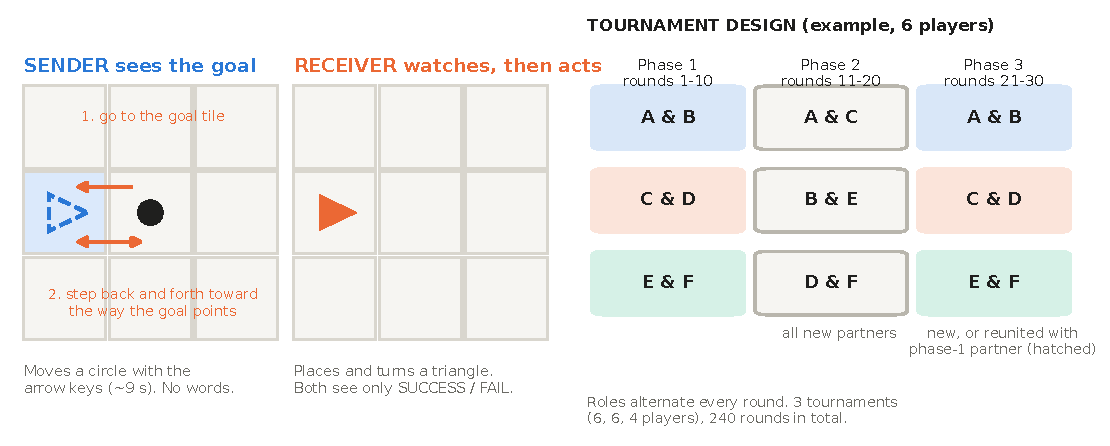
\includegraphics[width=\linewidth]{fig1_game}
\caption{\textbf{Task and design.} Left: an example Sender turn (go to the goal tile, then step back and forth toward the goal direction). Right: phases and re-pairing.}
\label{fig:game}
\end{figure}

\subsection{Readable move descriptions}
Each turn's key presses were compressed into readable steps (``went to top; wiggled top$\leftrightarrow$center $\times$5; long pause on top; time ran out''). Round-tripping all 240 real Sender turns through this format preserved the end tile in 100\% of turns and the hand-coded strategy in 93\%, but recovered the exact arrow-key sequence in only 59\% (intermediate tiles and pauses under one second are dropped).

\subsection{A single-turn embedding from LLM similarity judgments}
We did not want to rely on hand-coded strategy labels, which may be inaccurate. Instead, an LLM judge (GPT-6.1 Terra) saw three Sender turns (goal + moves) and named the one whose \emph{signalling strategy} was the odd one out, judged relative to each turn's own goal. We collected 2{,}500 such triplets over all 240 turns (balanced coverage; one third with all three turns sharing the exact goal) plus 1{,}560 two-choice partner/stranger probes, and fitted a three-dimensional embedding by maximum likelihood (softmax over squared distances). The judge gave the same odd-one-out answer on 84\% of reordered triplets; the embedding predicted 70\% of held-out triplets (chance 33\%). A new turn can be placed in the fixed embedding from about ten further judgments. Because the judge prompt listed example strategies, we repeated the whole procedure with the examples removed; results replicated with slightly lower validity.

For analyses of change over time we subtracted from each turn's vector the mean vector of all turns with the same goal (every goal occurred exactly eight times), so distances reflect style rather than goal difficulty.

\subsection{Validity benchmark}
Any single-turn representation was scored on fixed questions with known answers, each with candidates matched for the exact goal (chance 50\%): is a player's \emph{next} turn closer to their current turn than a same-goal decoy; is the current partner's turn closer than a stranger's (other tournament) or a same-tournament non-partner's; and does a turn's similarity to signals its Receiver decoded correctly before (versus failed) predict success (AUC).

\subsection{Counterfactual decoding}
A simulated Receiver (GPT-6.1 Terra) was given the game rules and five complete real games from other tournaments, written as moves, and asked where to place the triangle. \emph{Encoding}: a decoder with no player history read all 240 real Sender turns. \emph{Decoding}: within each tournament, each real player's history was truncated either at the end of phase 1 (early Receiver) or at the start of phase 3 (late Receiver); each version decoded eight phase-1 and eight phase-3 signals from \emph{other} players (never signals the player had actually received), giving a $2\times2$ design (512 decodes). Sender and Receiver effects are the main effects; the interaction measures a convention shared by late Senders and late Receivers. Confidence intervals resample Receivers.

\subsection{LLMs as models of players}
Leave-one-tournament-out, an LLM saw the rules, five complete real games from the other tournaments, and the target player's real game so far, and produced the player's next move: the steps of a Sender turn or a Receiver's tile and direction. We scored the strategy implied by the Sender's steps and the Receiver's reading of the signal against the real player, against a history-free baseline (43\% / 49\%). In closed-loop simulation, all players of a tournament were simulated and their histories grew from simulated rounds.

\section{Results}
\subsection{Success dips, then rises}
Real success was 29\%, 24\% and 49\% in phases 1--3. Separating phase-3 rounds by schedule, reunited pairs succeeded 57\% of the time and new pairs 40\% (both $n=40$), so part of the phase-3 jump reflects reunions; new partners still improved on phase 1.

\subsection{Signals get clearer; the phase-2 dip is a mismatch}
A single decoder with no history read phase-1, -2 and -3 signals correctly 36\%, 46\% and 61\% of the time (Figure~\ref{fig:success}). Phase-2 signals were \emph{more} decodable than phase-1 signals, yet real Receivers succeeded less often (24\%): Senders had moved to clearer signals that their new partners read differently. Among phase-3 signals, those sent to reunited partners were decodable 75\% of the time and those sent to new partners 48\%.

\begin{figure}[t]
\centering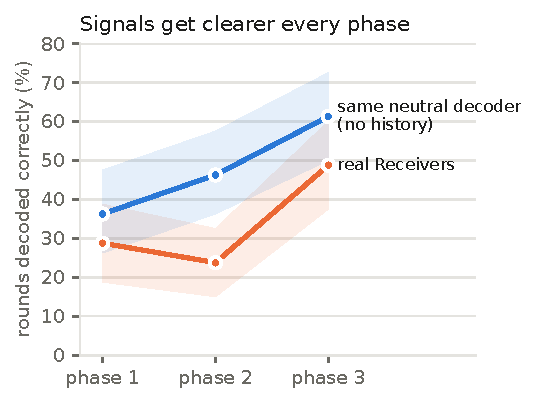
\includegraphics[width=0.55\linewidth]{fig2_success}
\caption{\textbf{Encoding improves.} The same history-free decoder reads real Sender turns from each phase (blue), versus the success of the real Receivers (orange). Bands: 95\% bootstrap CIs.}
\label{fig:success}
\end{figure}

\subsection{Encoding, not decoding}
In the $2\times2$ counterfactual (Figure~\ref{fig:cf}), late signals were decoded better than early ones by the same Receivers (+14 points, 95\% CI [+5, +22]); giving Receivers more history helped less and not reliably (+5 [$-$4, +14]); and late signals did not work especially well for late Receivers (interaction $-$1 [$-$12, +11]). The improvement is thus concentrated in what Senders produce, not in a private code shared with particular Receivers.

\begin{figure}[t]
\centering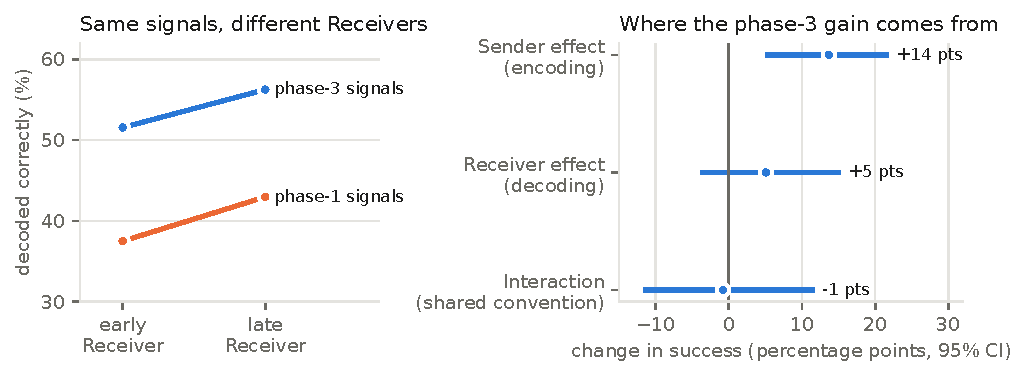
\includegraphics[width=\linewidth]{fig3_counterfactual}
\caption{\textbf{Counterfactual decoding.} Left: success for each combination of signal phase and Receiver history. Right: main effects and interaction (95\% CIs, Receivers resampled).}
\label{fig:cf}
\end{figure}

\subsection{What Sender turns look like}
The embedding supported only one robust split: turns that try to signal a direction versus ``still'' turns that just go to the goal (two clusters beat a one-blob null; more did not). A four-way description, written by reading raw turns without using hand codes, is still informative (Figure~\ref{fig:emb}): \emph{pointers} step back and forth between the goal and the neighbour in the goal direction (42\% success); \emph{right axis, unclear end} turns move along the correct line but leave which end is the ``head'' ambiguous (36\%); \emph{still/minimal} turns pause and mark the goal (42\%); \emph{busy/circling} turns loop through several neighbours and usually time out (16\%).

\begin{figure}[t]
\centering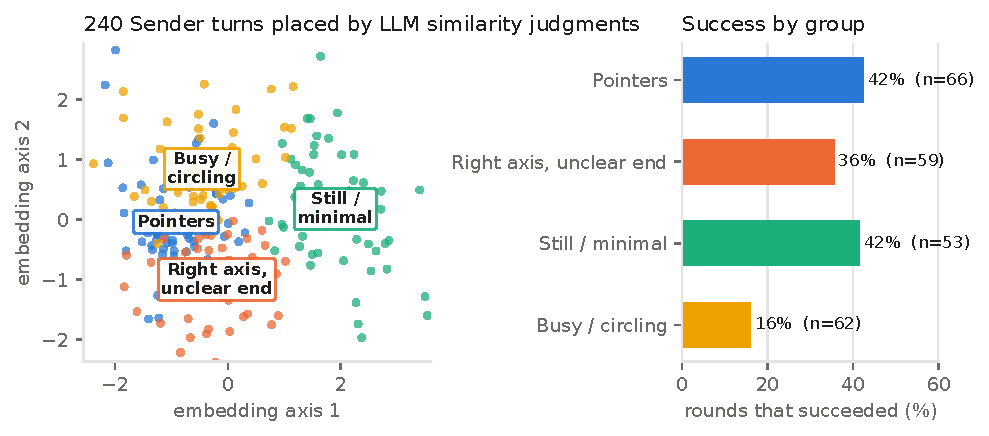
\includegraphics[width=\linewidth]{fig4_embedding}
\caption{\textbf{The single-turn embedding.} Left: all 240 Sender turns, coloured by a four-way k-means split and labelled with verbal descriptions. Right: success per group.}
\label{fig:emb}
\end{figure}

On the validity benchmark the embedding identified a player's next turn 60\% of the time, the current partner against a same-tournament non-partner 64\%, and predicted success with AUC 0.61 [0.53, 0.69]. Hand-coded strategy labels performed similarly (58\%, 53\%, 0.62); neither added predictive value beyond goal geometry (whether the goal direction points into the board) and phase. A confound check showed that the success signal reflects generic signal quality: similarity to successes and failures of players in \emph{other} tournaments predicted success as well as the Receiver's own history did. Direct pairwise judgments retained more information than the three-dimensional embedding (for example, 73\% versus 60\% on next-turn identification).

\subsection{Partners pull each other's style}
In goal-removed embedding space, partners' turns were always closer to each other than to non-partners' (Figure~\ref{fig:conv}, left). All distances fell in phase 2, including between players in different tournaments who never met, which points to a shared shift at that stage rather than social copying; in phase 3 styles spread again except between current partners. Regressing each player's next turn on their own previous turn and their current partner's latest turn gave weights of 0.25 ($p<.001$) and 0.13 ($p=.002$); substituting a random non-partner gave $-$0.08 (Figure~\ref{fig:conv}, right). The partner pull was present in phases 1 (0.16, $p=.01$) and 3 (0.17, $p=.04$) and absent in phase 2, and it replicated with the unprompted judge (0.14, $p=.009$). An LLM judge could not tell which tournament a turn came from (50\%), so we find pairwise pulls but no group signature. We found no reliable lock-in: the size of a player's turn-to-turn change did not shrink with games played together once phase was controlled (slope $+0.001$ per game, $p=.96$), and was only slightly smaller after successes (1.60 vs 1.76).

\begin{figure}[t]
\centering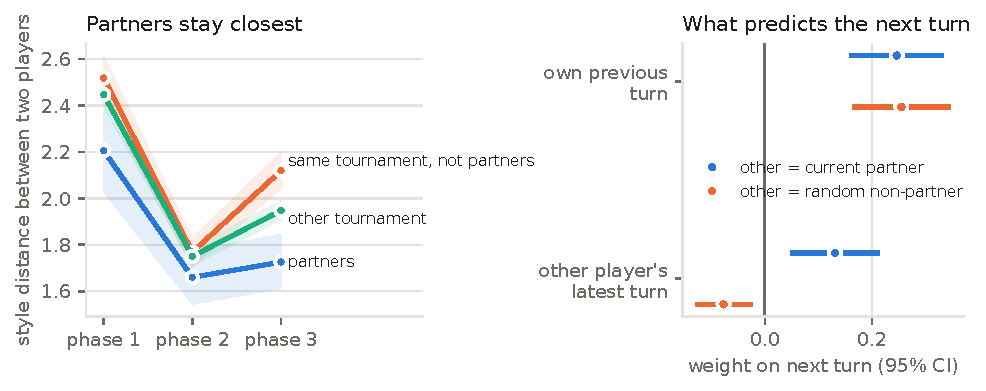
\includegraphics[width=\linewidth]{fig5_convergence}
\caption{\textbf{Convergence.} Left: style distance between two players' turns in the same phase. Right: weights on a player's next turn (95\% CIs clustered by player).}
\label{fig:conv}
\end{figure}

\subsection{LLMs as models of players}
Given each player's real history, GPT-6.1 Terra predicted the Sender's strategy 57\% of the time and the Receiver's reading 63\% (history-free baseline 43\% / 49\%), ahead of Claude Sonnet 5.5 (50\% / 57\%) and Claude Haiku 5.5 (41\% / 43\%, below baseline; Figure~\ref{fig:llm}, left). Terra's exact Receiver placements matched 42\%, against 38\% for the rule ``sender's last tile, pointing the way the wiggle points''. A judge preferred Terra's predicted turn over the player's previous turn as a match to the actual turn 70\% of the time, against 53\% for a same-goal turn by another player (goal-match control). With the goal held fixed, however, Terra's prediction of the next turn was judged closer to the current turn than the player's \emph{real} next turn was (58\%, $p=.013$): the model under-predicts how much people change. Consistently, LLM players were too clean (ending on the goal 99\% vs 92\%) and closed-loop simulations did not reproduce the dip-and-rise. % SIMULATION NUMBERS: filled in below
In closed loop (GPT-6.1 Terra playing every player of a held-out tournament on its real schedule, histories growing from simulated rounds; 12 sessions, 4 per tournament, 960 rounds), simulated pairs succeeded 48\%, 68\% and 60\% of the time in phases 1--3 against 29\%, 24\% and 49\% for the real players. Simulated Senders always ended on the goal tile (100\% vs 92\%), and rather than dipping, success peaked in phase 2, where simulated Receivers read signals as intended 65\% of the time (real 30\%). The simulated groups thus coordinate far more easily than people do and miss the partner-switch cost.


\begin{figure}[t]
\centering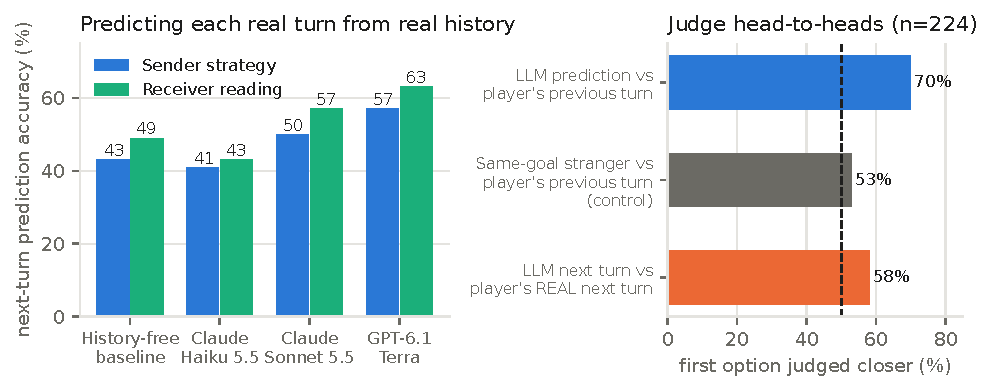
\includegraphics[width=\linewidth]{fig6_llm}
\caption{\textbf{LLMs as models of players.} Left: next-turn prediction accuracy from real history (leave-one-tournament-out). Right: judge head-to-heads on 224 Sender turns.}
\label{fig:llm}
\end{figure}

\section{Discussion}
Across methods, the improvement in this game is best described as Senders learning to produce signals that are legible to anyone, while Receivers adapt more slowly. The early cost of switching partners is not worse signalling but a mismatch between a Sender's newer, clearer signal and a new partner's reading of it, consistent with accounts in which successful communication depends on conceptual alignment between interlocutors \citep{stolk2016}. Styles are pulled toward the current partner, but within our short sessions this did not add up to a group convention.

\paragraph{Limitations.} The sample is small (16 players). Phase-3 reunions in two tournaments inflate the phase-3 gain and are confounded with tournament. The counterfactual Receivers are simulated, and LLM simulators are too stable, so the decoding effect may be underestimated. The embedding judge is an LLM whose prompt originally listed example strategies; the unprompted replication reduces but does not remove this concern. Single-turn embeddings lose information relative to direct judgments.

\paragraph{Next steps.} Run more tournaments with a balanced schedule (no reunions); embed Receiver turns so that Sender--Receiver fit can be measured from single rounds; and test whether fine-tuned or better-calibrated models can reproduce human variability in closed loop.

\bibliographystyle{unsrtnat}
\bibliography{refs}
\end{document}
